% CREATED BY DAVID FRISK, 2015
\chapter{Methods}


This chapter will describe methods and definitions of generating guidelines for brickwork on a surface that is a result of form finding. Definitions and procedure will be derived from the theory described in the previous chapter.   


\section{General}

The method will be based on geodesic coordinates and polar geodesic coordinates on a surface that has been described in \ref{sec:geoCord}. The main idea is to make a discrete formulation of the continuous definition of geodesics and in extension a discrete formulation of the geodesic coordinates. This will be implemented on a continuous surface using a discrete solver for dynamic problems, called dynamic relaxation, describe in section \ref{DR}. This will be implemented in a parametric design environment and part of a parametric design scheme described in \ref{dScheme}. The process and generation of geodesic coordinates will be described in the following chronological order of the implementation:
\vspace{5mm}
\begin{enumerate}
\item Form Finding, generate a form that fulfills equilibrium.
\item Generation of geodesic points on the surface.
\item From the geodesic points orthogonal trajectories will be constructed 
\end{enumerate}
\vspace{5mm}
The implementation is a bit different between the two types of geodesic coordinates but the main idea is similar.

\section{Discrete definitions}
This section will describe how this thesis interprets the continuous definitions in Classical Differential geometry to Discrete definitions. 
\subsection{Definition of discrete geodesic points}

The continuous definition of a geodesic curve is that in each point along the curve the geodesic curvature is zero, i.e curve can only be curved in the normal direction. This could be interpreted as the tangent of the curve and the normal forming a plane. For a discrete definition one can imagine three points on a surface where the points are connected through two vectors,A and B, starting in the middle point, see figure below. If the normal of the middle point and the two vectors lies in the same plane the middle point is defined as a geodesic point. This means that the cross product of A and B is orthogonal to the normal and the projection on the normal would be zero, i.e the geodesic component is zero. And for a small enough distance on the surface a collection of geodesic points will form a geodesic curve.

\begin{figure}[H]
\centering
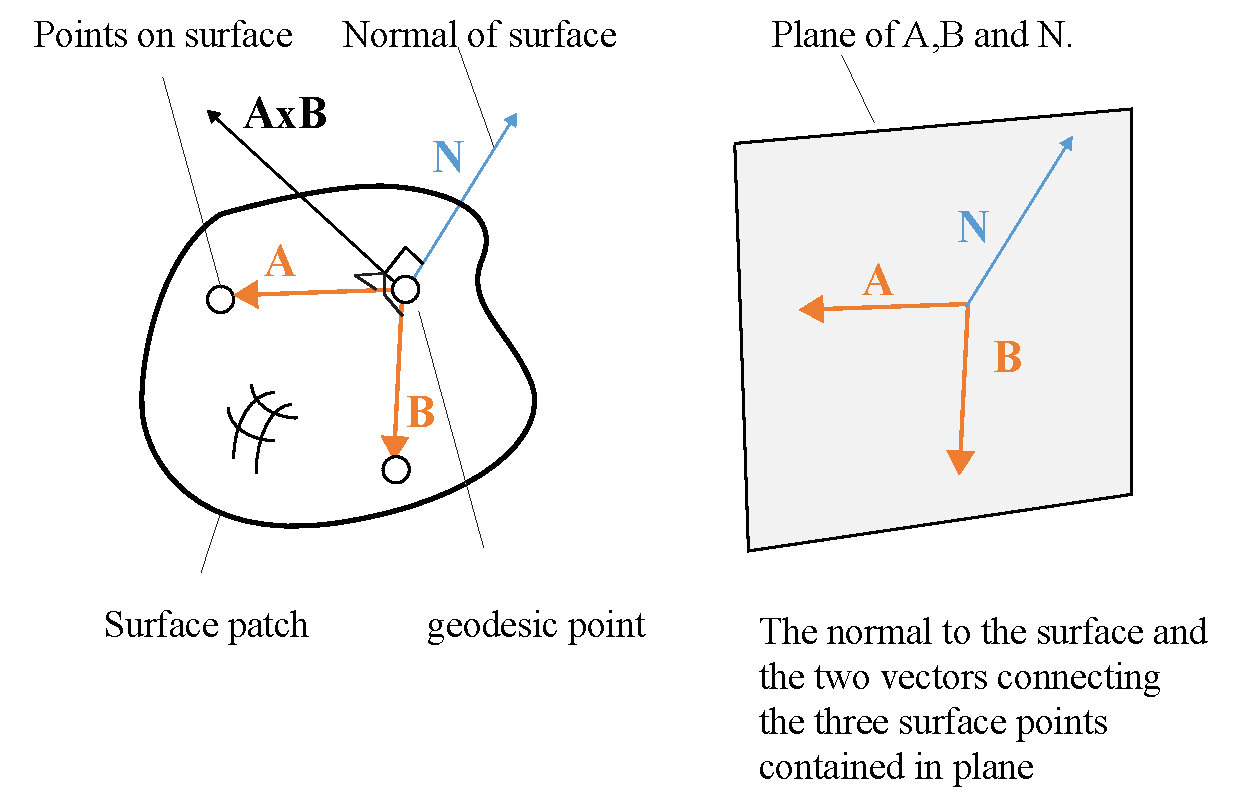
\includegraphics[width = 0.8\linewidth ]{figure/Method/defintionGeodeiscPoint.pdf}
\caption{http://web.mit.edu/hyperbook/Patrikalakis-Maekawa-Cho/node29.html}
\end{figure}

\subsubsection{Physical interpretation}

Making a physical interpretation of the geodesic point is by defining a discrete curve as a set of connected springs. The springs are of the same initial length with a pre-tension, that is the same for all springs, is applied in the springs. Isolating the node one will find a spring force in the direction of the connected springs. Adding these two forces results in a resultant force in that node. When the resultant force can be described in  the normal of the surface in that point, the geodesic force component is zero. This is the physical definition of a geodesic point which equivalent the discrete defintion above.

\begin{figure}[H]
\centering
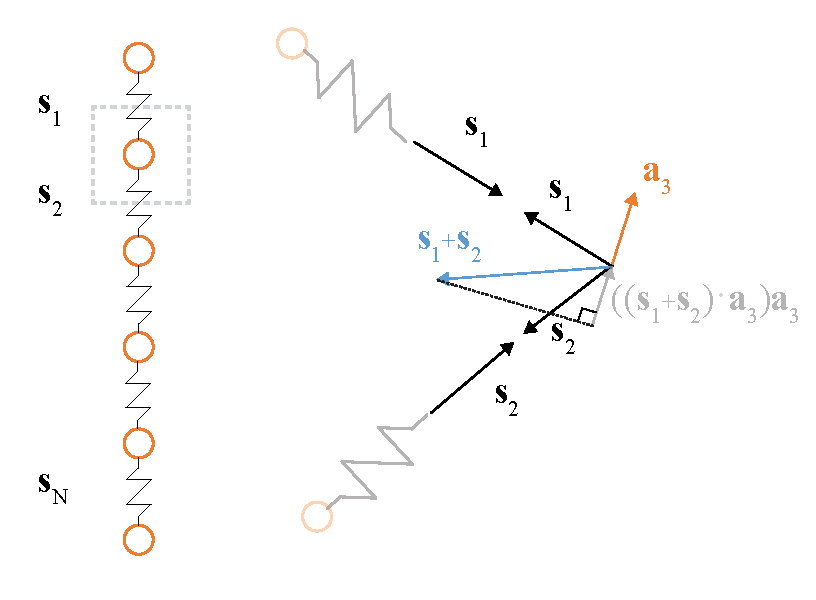
\includegraphics[width = 0.8\linewidth ]{figure/Method/GeodesicDR.pdf}
\caption{http://web.mit.edu/hyperbook/Patrikalakis-Maekawa-Cho/node29.html}
\end{figure}

\subsection{Definition of discrete geodesic coordinates}

There are, as mentioned, two types of geodesic coordinates:

\begin{enumerate}
\item General geodesic coordinates
\item Polar geodesic coordinates
\end{enumerate}

The main properties of a geodesic coordinate system is that it is formed of two sets of curves, the first is geodesics and the second is orthogonal trajectories that intersects the geodesics at right angles with an equal distance along the geodesics.

\vspace{5mm}

\subsubsection{Definition of discrete Polar geodesic coordinates}

The main difference is between polar and general geodesic coordinates is that in the polar coordinates the geodesics has its origin in the same point, the pole, and radially distribute from that point. The pole will play an important part for the discrete definition since the continuous definition states that at an equal distance along all geodesics we will find an orthogonal trajectory measured from the pole, see figure below.  Applying the same logic to a set of geodesic points, i.e the geodesic points are distributed at an equal distance from the pole and adjacent points as in figure below, the trajectories will not necessarily be orthogonal. This definition states that for a sufficient number of sets of geodesic points the trajectories will converge towards a continuous orthogonal trajectory. 

\begin{figure}[H]
\centering
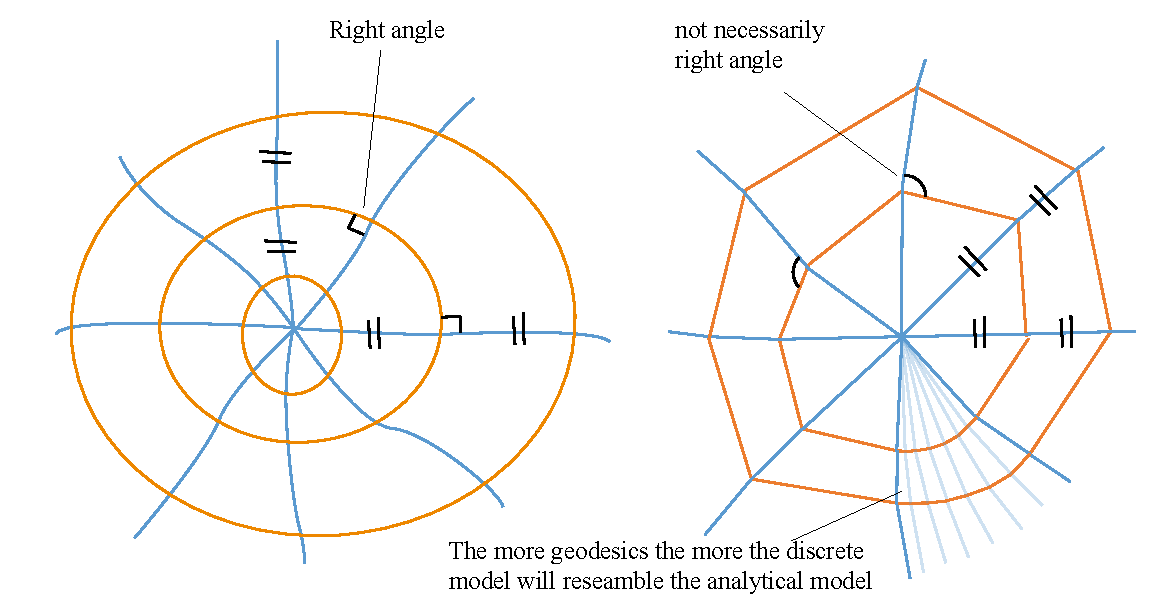
\includegraphics[width = 1.0\linewidth ]{figure/Method/polargeo.pdf}
\caption{To the right the continuos defition of polar geodesic coordinates and to the right a discrete interpretation. The discrete definition in this paper states that following continuous definition the discrete will at sufficient amount of sets of geodesic points the discrete will converge towards the continuous model}

\end{figure}

\subsubsection{Definition of discrete General Geodesic Coordinates}

For general geodesic coordinates it lacks a common starting points for the geodesics. It is therefore necessary to add a condition to the one of equal length. The angles that are created when two adjacent points from two sets geodesic points are of similar angle $\alpha$ , see figure below, it will resemble a orthogonal trajectory, and fore an infinite amounts of geodesics sets it will be continuous orthogonal trajectory. 

\begin{figure}[H]
\centering
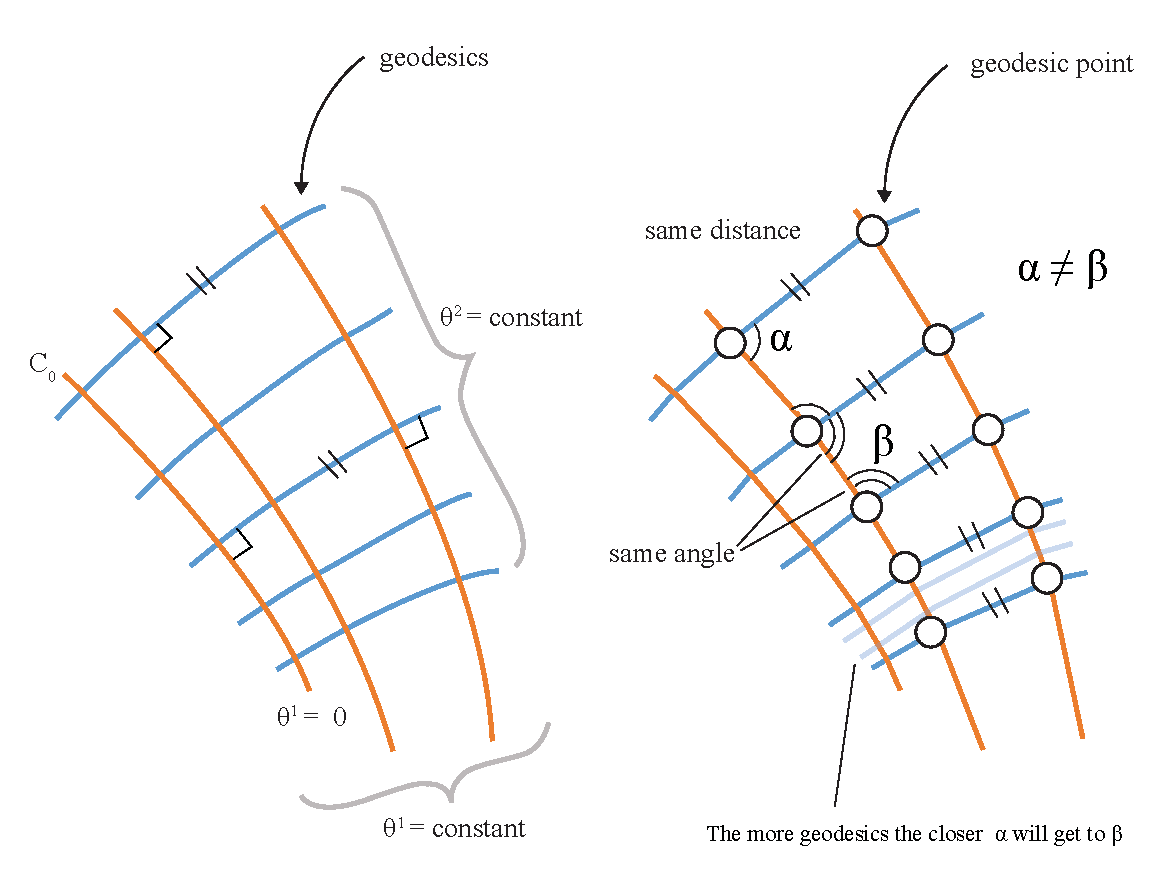
\includegraphics[width = 1.0\linewidth ]{figure/Method/diiscreteGeodesicCoord.pdf}
\caption{To the right the continuos defition of polar geodesic coordinates and to the right a discrete interpretation. The discrete definition in this paper states that following continuous definition the discrete will at sufficient amount of sets of geodesic points the discrete will converge towards the continuous model}
\end{figure}




\section{Separated form and geodesic generation}

This method as it states separate the form generation and the geodesic pattern generation. Therefore it gives more freedom in the sense that the form-generation can be focused on spatial and structural requirements. The method can be divided into three different stages.

\begin{enumerate}
\item Generate a form that satisfies equilibrium for masonry structures
\item Generate geodesics, that does not cross each other, on that surface
\item Generate the orthogonal trajectories that cuts the geodesics in equal length curves. 
\end{enumerate}

\subsection{Model preparation and Form-finding}


For this purpose it is only interesting to use numerical form-finding methods. It should be possible to choose whichever that pleases you where you can apply vertical loads for self-weight. For masonry structures it is important though that all forces and stresses acts in compression. The most suitable method for masonry structures is the TNA but it not implemented in a parametric environment, so far, so in this case traditional FD or DR method will be used. The numerical solvers implemented generates a set of curves or a mesh. To generate a surface from this a standard feature in \textit{Grasshoper3d} is used to convert a discrete surface to a mathematical surface.



\begin{figure}[H]
\centering
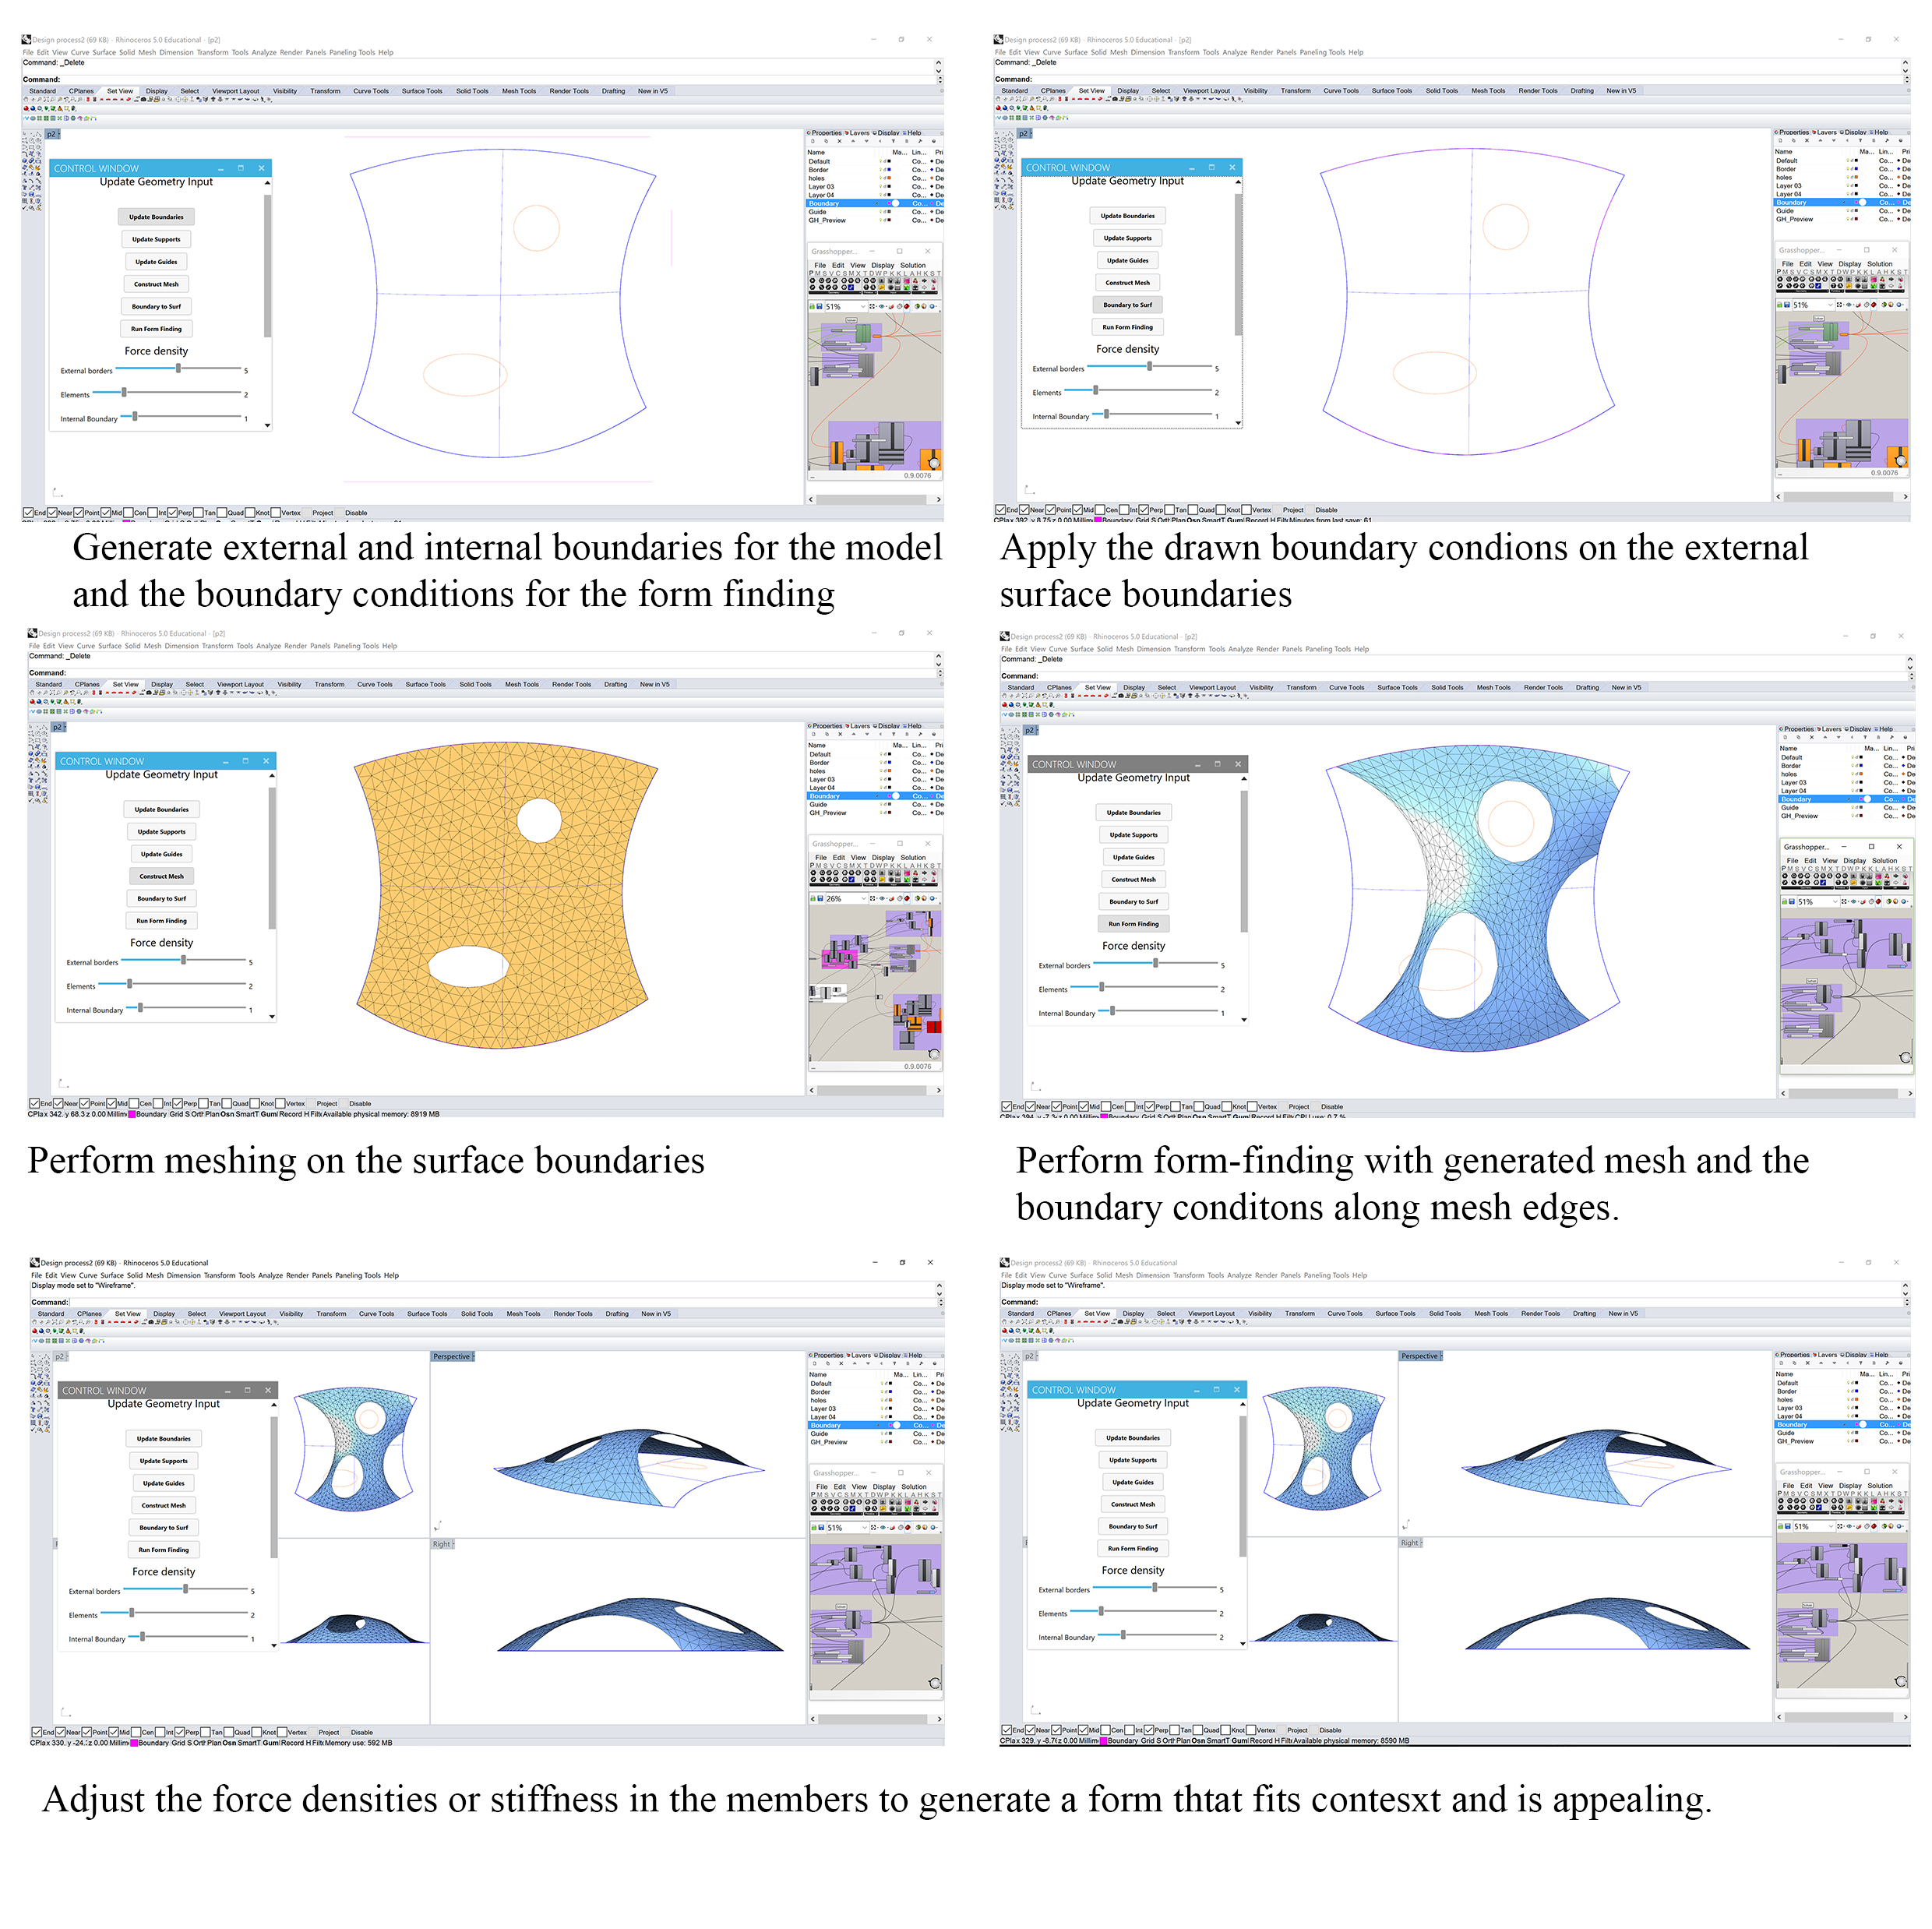
\includegraphics[width = 1.0\linewidth ]{figure/Method/ModelGen.jpg}
\end{figure}



\subsection{Geodesics}



\subsubsection{Generation of geodesic points}
It is possible to generate geodesics on a surface using for instance a DR or PS solver. An important bit to understand is that this is discrete solving procedure for a continuous problem. This contradiction is not very strange to engineers to since FEM is a discrete formulation of a structural system or element. The main idea is to model the geodesics as a set of springs that can move on a continuous smooth surface.In the picture below it shows the curve discretizied into springs. The springs should only be loaded with a pre-tensional force. The goal is to reduce the force component in the geodesic direction,i.e the geodesic curvature. It is possible to check this geodesic condition geometrically for each point, or node in this case. The cross product of the vectors in the same direction of the springs  should be perpendicular to the normal in the node point, see the right part of figure below.




\vspace{5mm}


\begin{enumerate}
\item Decide the end points of the geodesics on the surface.
\item Generate an initial curve that lies on the surface




\item Discretize  the curve into segments, small enough to resemble the curve properties, of the same length. This segments will be the springs in the DR or PS algorithm.



\item Apply the same pretension in all elements and ensure that the nodes move along the surface, this can be done by either a force or just moving the point to surface in each iteration. 
\item Start the solver, and for each iteration check the geodesic requirement for each point, or node. When all nodes are geodesic points then solution has converged and the iterations end. The geodesic points should, due to the equal inital length and tension, should still have equal distance.The moved points are orange in the picture below.


\end{enumerate}

\begin{figure}[H]
\centering
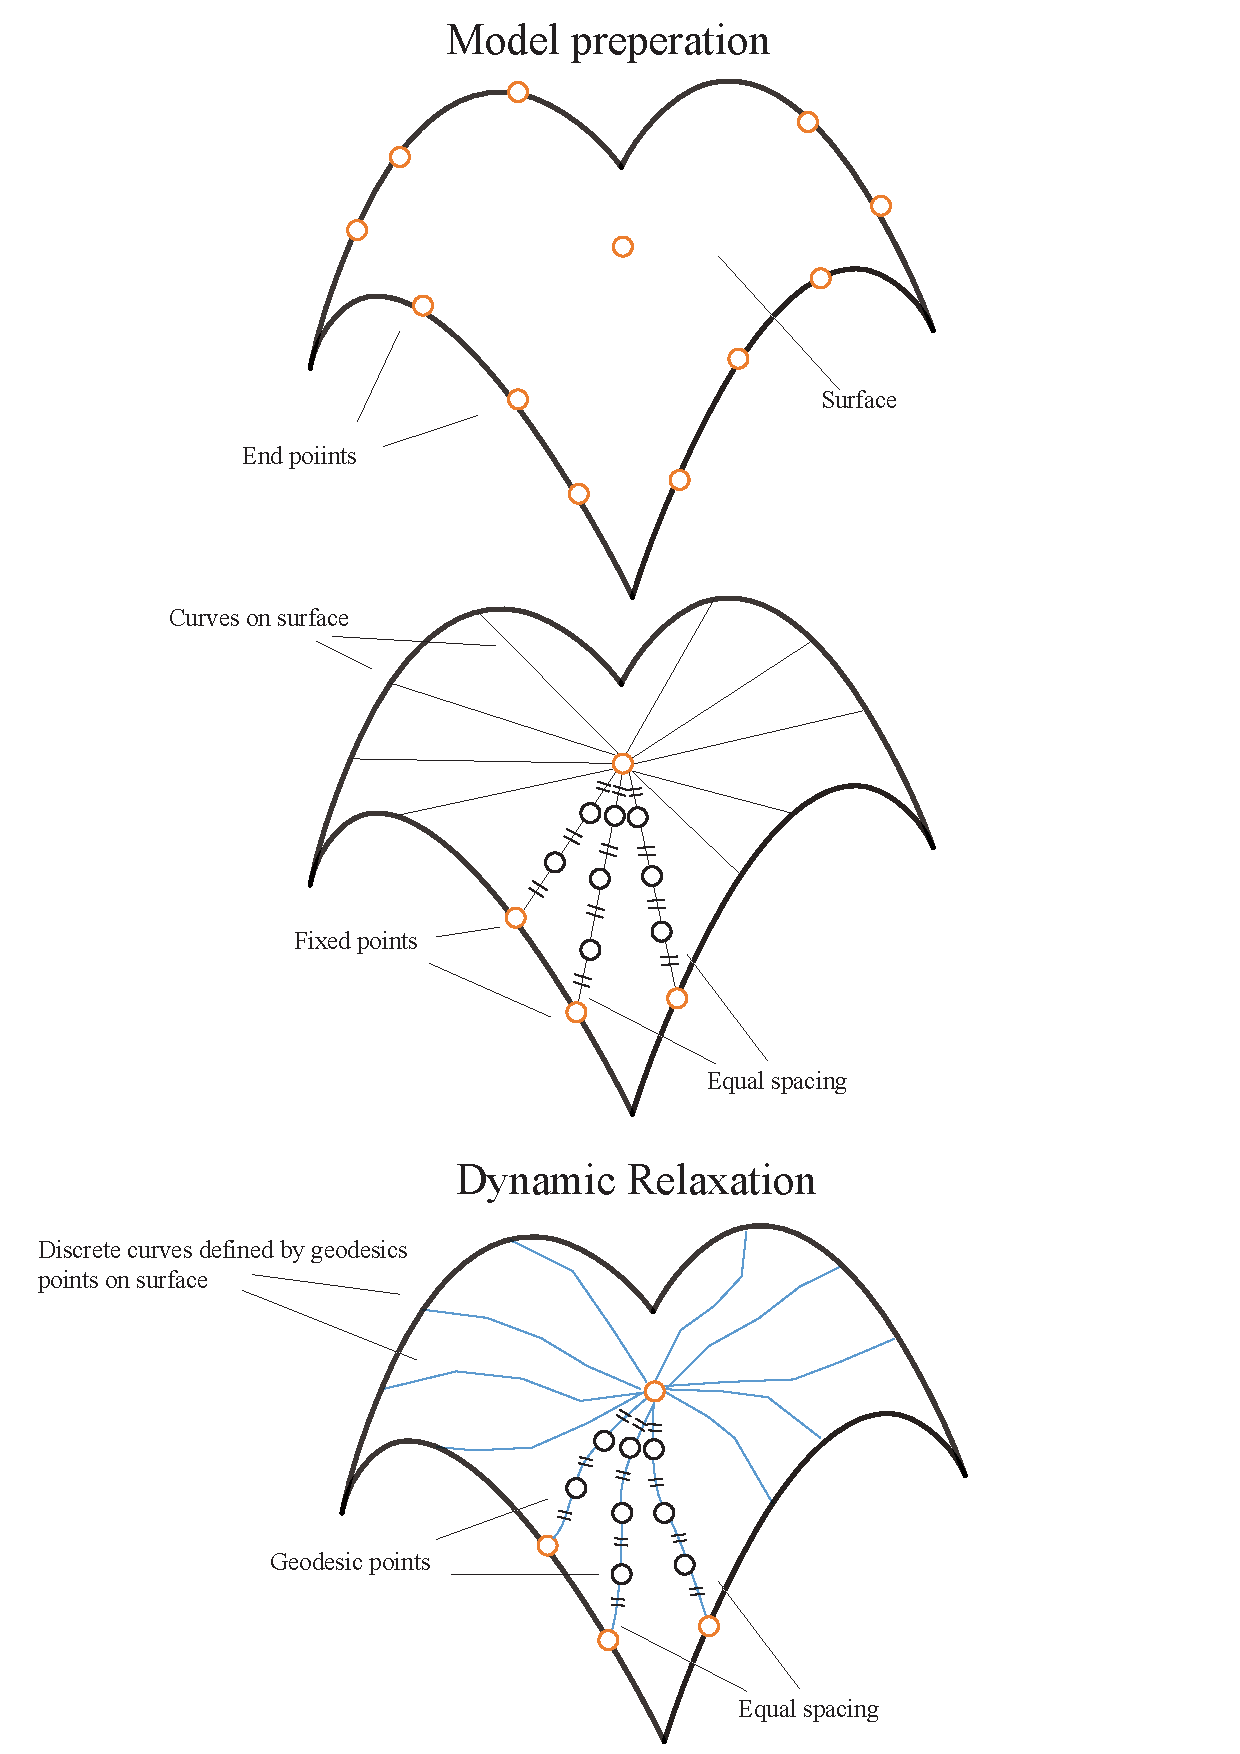
\includegraphics[width = 1.0\linewidth ]{figure/Method/Stepps.pdf}

\end{figure}


\subsection{Generation of the orthogonal trajectories}

Depending on how the geodesics have been chosen an generated different methods can be applied to generate the orthogonal trajectories. The two different possibilities refer to

\begin{enumerate}

\item Geodesic starting from a point, referring to a polar geodesic coordinate system, see figure \ref{fig:polargeo}
\item Arbitrary geodesics, referring to a geodesic coordinate system  as in figure \ref{fig:geodesicCoord}
\end{enumerate}
\vspace{5mm}
The first case is the less complicated of the two. The generated geodesic points are spaced with the same distance and all of them starts in a center point. Since the starting point is the same moving equal distance in the geodesic directions a orthogonal trajectory shall pass that point, in continuous theory as figure \ref{fig:polaralg}a). This is though, wort to mention again,  discrete approach, generated in previous steps are just a collection of geodesic points rather than a analytical curve. For a small enough distance the discrete solution approaches the continuous solution. Connecting the points generating the orthogonal trajectories as in figure \ref{fig:polaralg}b), they are not necessarily orthogonal, but with more geodesics the solution converges towards the right angle. 

\begin{figure}[H]
\centering
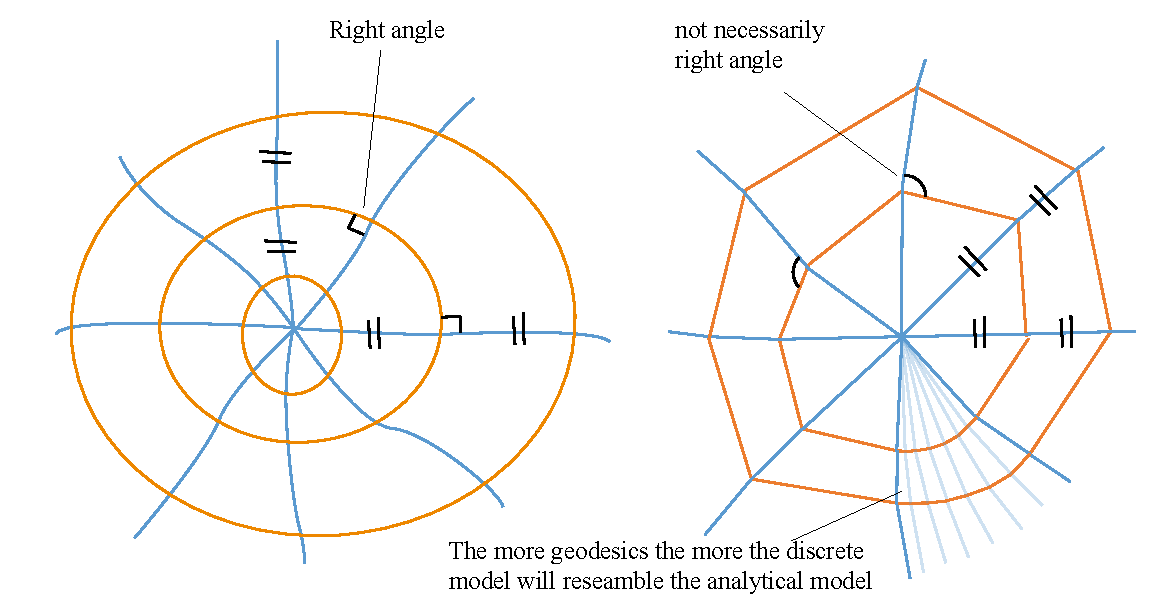
\includegraphics[width = 1.0\linewidth ]{figure/Method/polargeo.pdf}
\caption{http://web.mit.edu/hyperbook/Patrikalakis-Maekawa-Cho/node29.html}
\label{fig:polaralg}
\end{figure}


The second case is a bit more complicated since there is no reference that are equal to all geodesic lines, as the starting point in polar geodesic coordinate case. Referring to the statement of Struik which is quoted in section \ref{sec:geoCord}, meaning that the entire orthogonal trajectory set can be found from on orthogonal trajectory. This implies that finding that first will be the main task and the others will follow quite easily. In the figure \ref{fig:geoAlg} below the procedure is described. The goal is to make the angles $\alpha$ and $\beta$ equal, and as close as possible to 90 degrees. To make this possible the end lengths of the geodesics are allowed to vary. This can be done using DR as in the previous geodesic generation. The internal springs will be modelled with similar stiffness and tension. The end springs will be modelled with a different stiffness than the internal springs. To only allow elongation the internal springs should be modelled as very stiff compared to the end springs.


\begin{figure}[H]
\centering
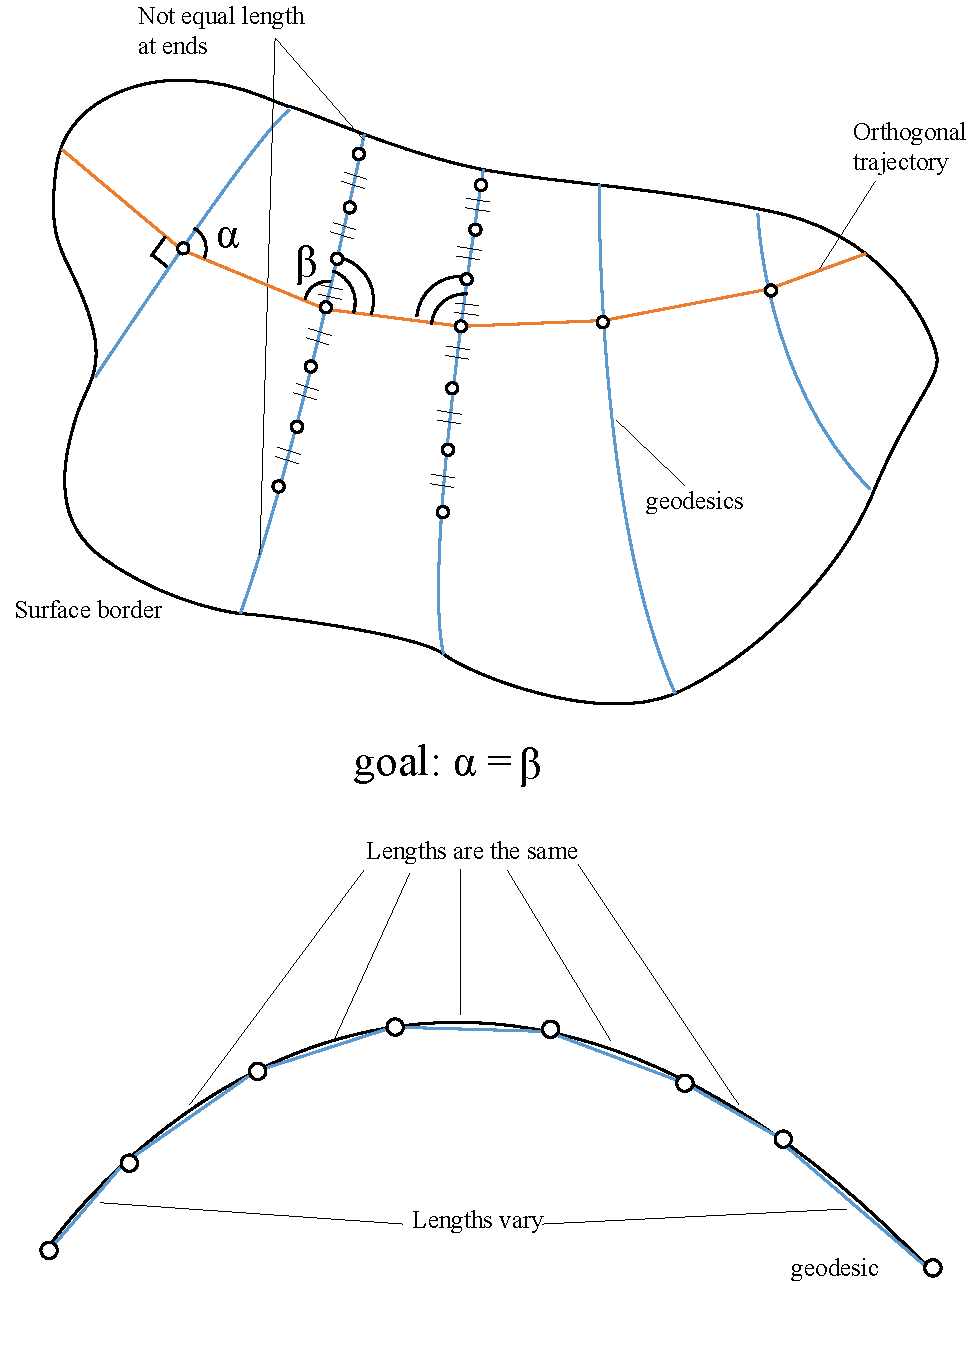
\includegraphics[width = 0.8\linewidth ]{figure/Method/GeodesicCoord.pdf}
\caption{http://web.mit.edu/hyperbook/Patrikalakis-Maekawa-Cho/node29.html}
\label{fig:geoAlg}
\end{figure}


